\chapter{Úvod}
  Odtlačky prstov sú komplikovanou spleťou cestičiek, ktoré sa navzájom krížia, spájajú a ukončujú, vytvárajú slepé uličky alebo diaľničné uzly.
  Kombinácie týchto vlastností cestičiek vytvárajú unikátny podpis ich vlastníka. Tieto cestičky, nazývané papilárne línie, sú pozorovateľné
  voľným okom a sú kategorizovateľné, čo znamená, že ich unikátnosť je možné využívať v rôznych smeroch bezpečnosti. Spočiatku sa odtlačky prstov
  využívali v kriminalistike, kde rýchlo nabrali na popularite a ich využitie bolo čím ďalej, tým viac rozšírené. S~príchodom výpočtových systémov
  sa ich analýza začala automatizovať, čo znamenalo digitalizáciu záznamov, prispôsobovanie rôznych matematických konštrukcií pre zjednodušenie ich
  analýzy počítačmi a celkové rozšírenie znalostí o odtlačkoch prstov. 
  
  Koncom minulého storočia sa navrhlo množstvo rôznych prístupov k spracovaniu odtlačkov prstov, ktoré boli časom vylepšené, prípadne integrované
  medzi sebou. Základné princípy automatizovanej analýzy sú však zväčša nemenné. Väčšina metód sa spolieha na viackrokové predspracovanie
  vstupnej snímky a následnú analýzu upravenej snímky. Predstavením základných pojmov skúmania odtlačkov prstov a takýmto spôsobom ich analýzy
  sa zaoberá kapitola \ref{kap:odtlacok}.

  Digitalizácia záznamov odtlačkov prstov v Spojených štátoch amerických predstavovala veľkú výzvu pre dátové skládky tamojších kriminalistických orgánov, pretože 
  metódy kompresie snímok neboli v tej dobe prispôsobené zachovávaniu detailov potrebných pre bezproblémovú analýzu odtlačkov prstov 
  po kompresii. Ako riešenie Americký Federálny úrad pre vyšetrovanie (FBI) implementovalo novú metódu kompresie snímok založenú na diskrétnej vlnkovej transformácii
  vo formáte vlnkového skalárneho kvantovania (WSQ). Súborom WSQ a~spôsobu kompresie v tomto formáte sa venujem v kapitole \ref{kap:wsq}.

  Vzhľadom na množstvo rôznych úkonov spojených s analýzou odtlačkov prstov je pri študovaní týchto úkonov nápomocné mať vizuálne pomôcky
  pre demonštráciu procesov s nimi spojených. Obrázky a náčrty v študijných materiáloch sú samozrejme veľkou pomôckou, avšak nemusia vždy
  poskytnúť tie informácie, ktoré študent potrebuje. Výstup tejto práce má za cieľ poskytnúť aplikáciu, ktorá je schopná reprodukovať
  niektoré najbežnejšie úkony predspracovania a analýzy snímok odtlačkov prstov tak, aby užívateľovi demonštrovali význam jednotlivých úkonov
  interaktívnym spôsobom na snímkach dodaných samotným užívateľom. Návrh aplikácie je popísaný v kapitole \ref{kap:navrh_appky}.
  
  % //TODO: ak bude dalsia kapitola, tak v kratkosti este popisat aj tu

\chapter{Odtlačok prsta} \label{kap:odtlacok}
  Koža sa skladá z troch častí: pokožka (epidermis), zamša (dermis) a podkožné väzivo (hypodermis). Výbežky a údolia štruktúr na končekoch prstov,
  naprieč dlaňami a chodidlami
  sú zakorenené v prostrednej časti, dermis, kde sa prelínajú s primárnymi výbežkami (nachádzajúcimi sa pod povrchovými výbežkami) a sekundárnymi
  výbežkami (nachádzajúcimi sa pod povrchovými údoliami) čo im dodáva pevnosť. Tieto štruktúry sú nazývané papilárnymi líniami.
  V časti dermis a hypodermis korenia aj potné žľazy, ktoré na povrchu kože vyústia do pórov \cite{FingerprintSrcBook}. Papilárne línie, potné žľazy
  a iné štruktúry na povrchu kože sa v následku dotyku nejakého povrchu na ňom odtlačia a zanechajú po sebe \uv{mapu}, 
  ktorej sa všeobecne hovorí odtlačok prsta.

  Každý človek na svete je unikátne identifikovateľný podľa odtlačkov prsta. Ako prvý publikoval význam papilárnych línií pre identifikáciu
  jednotlivcov Henry Faulds. V roku 1880 publikoval článok v žurnále \emph{Nature} informujúci výskumníkov o jeho zisteniach o unikátnosti
  a permanencii papilárnych línii. V danom článku opísal dva konkrétne prípady, kde boli využité odtlačky prstov na individualizáciu osôb a navrhol
  používanie takéhoto spôsobu identifikácie na miestach činu. V roku 1892 sir Francis Galton napísal prvú knihu o odtlačkoch
  prstov \emph{Finger Prints}, v ktorej definoval a pomenoval špecifické markanty odtlačkov prstov \cite{FingerprintSrcBook}.
  
  %Toto je vďaka vývojovým procesom,
  %ktoré sa začnú v ľudskom embryu približne jedenásť týždňov od oplodnenia, keď sa začnú na prstoch embrya vytvárať papilárne línie.
  %Tieto procesy, podobne ako napríklad procesy, ktoré zabezbečujú vývoj žíl a ciev v ľudskom tele, sú pre každého jedinca neidentické.
  %Papilárne línie sú tvorené vonkajšou vrstvou kože, epidermou, na prstoch rúk a nôh. Po úplnom vyvinutí papilárnych línií sa po celý život jedinca
  %bez vonkajšieho zásahu nijak zásadne nezmenia. Odtlačok zanechaný na povrchoch materiálov osobou, ktorá sa ho dotkne je obecne nazývaný odtlačkom prstu.
    
  \section{Klasifikácia odtlačkov prsta}
  Prvú klasifikáciu vzorov tvorených papilárnymi líniami na končekoch prstov je možné nájsť v dizertácii českého profesora Jana Evangelisty Purkyně
  z roku 1823 \cite{FingerprintSrcBook}. Začiatkom 20. storočia Edward Henry vyvinul klasifikačný systém, ktorý bol neskôr použitý ako základ pre systém
  automatizovanej identifikácie odtlačkov prsta (AFIS). Tento systém bol vyvinutý FBI pre extrakciu markantov odtlačkov prstov automatizovanými metódami
  za pomoci počítačov.

  Odtlačky prstov je možné skúmať na rôznych úrovniach detailu. Vlastne sa jedná o mieru špecifickosti, podľa akej zaraďujeme vlastnosti
  papilárnych línií na jednotlivých odtlačkoch prstov.

  \textbf{Na prvej úrovni}, najglobálnejšej, sa jedná o takzvané singularity, ktoré sa prejavujú ako náhle zmeny v priebehu papilárnych línií. Tieto 
  zmeny môžu byť časté zakončenia alebo rozdvojenia línií na malej ploche, ktoré tvoria \emph{delty} alebo ostré záhyby v líniách, 
  ktoré tvoria \emph{špirály} a \emph{slučky} \cite{Handbook}. 

  Obecne je na najvyššej úrovni každý odtlačok prsta zaraditeľný do jednej zo šiestich hlavných tried na základe obrazca tvoreného odtlačkom prsta:
  \begin{itemize}
    \item oblúk
    \item špirála
    \item ľavá slučka
    \item pravá slučka
    \item klenutý oblúk
    \item dvojitá slučka \cite{Henry}.
  \end{itemize}
  Klasifikačný systém AFIS využívaný v FBI rozlišuje prvé štyri spomenuté \cite{FingerprintSrcBook}.
  Triedy odtlačkov prsta nie sú v ľudskej populácii distribuované rovnomerne.
  Slučky majú najväčšie zastúpenie a sú pozorovateľné až u 61\% obyvateľstva, špirály u 34\% obyvateľstva a oblúky u zvyšných
  5\% obyvateľstva \cite{sciencing}.

  \textbf{Na druhej úrovni}, taktiež nazývanej lokálna úroveň, pozorujeme markanty. Markanty sú útvary tvorené ukončením alebo
  vetvením papilárnych línií. Tieto útvary je možné detegovať, identifikovať a klasifikovať a následne využiť pri analýze odtlačkov prstov.
  Klasifikácia markantov je obšírnejšia, než triedenie odtlačkov prstov, pričom medzi základné markanty zaraďujeme:
  ukončenie, jednoduchá  vidlička, dvojitá vidlička, trojitá vidlička, hák, kríženie, bočný kontakt, bod, interval,
  jednoduchá špirála, dvojitá špirála, jednoduchý most, dvojitý most a~priesečná línia \cite{Drahansky}.
  Kvôli veľkému množstvu rôznych typov markantov a zložitosti ich rozlíšeniu automatizovanými systémami sa počet rozlišovaných markantov v mnohých
  situáciách redukuje, pričom sa často využívajú iba prvé dva druhy markantov.

  \textbf{Na tretej úrovni}, najlokálnejšej, sa rozoznávajú detaily kože a atribúty papilárnych línií. Na tejto úrovni je možné pozorovať
  póry, šírku papilárnych línií, jazvy a poranenia kože, kožné ochorenia, atp. Dlhú dobu sa pri automatizovanej analýze detaily na tejto úrovni
  nespracúvali z dôvodu, že pri nižších rozlíšeniach snímok, typicky pod 1000ppi (bodov na palec - jednotka používaná napr. pri snímačoch a skeneroch),
  tieto detaily nie sú pozorovateľné \cite{Handbook}.
  %TODO: v skratke popísať ako sa teraz využívajú póry a info tretej úrovne v dnešnej dobe  
  %       napr. https://www.sciencedirect.com/science/article/pii/S0167865518303350

  \section{Spracovanie a analýza snímok odtlačkov prstov} \label{sec:analyza}
  %V súčasnosti automatizované analyzátory odtlačkov prstov vyžadujú úpravu zdrojových snímok. Surové snímky odtlačkov totiž nie sú vhodné pre
  %extrakciu informácí pomocou algoritmov. Skôr, než sa zo snímok môžu začať extrahovať vlastnosti ako singularity a markanty je potrebné snímku
  %spracovať tak, aby sa so snímkou pracovalo jednoduchšie pri samotnej analýze.

  %Medzi hlavné kroky spracovania vstupnej snímky patria zníženie šumu snímky, zvýšenie kontrastu a binarizácia snímky a ztenšenie línií.

  Metódy spracovania a analýzy odtlačkov prstov sa líšia na základe požadovanej aplikácie analyzátora. Napríklad pri zabezpečovaní mobilných telefónov
  sa nekladie až taký dôraz na kvalitu analýzy ako napríklad v kriminalistike, a teda sa mnohé časti analýzy preskočia, prípadne
  sa im nevenuje veľká pozornosť za účelom zrýchlenia systému. Avšak hlavná kostra analýzy je vždy relatívne nemenná.

  % //TODO: mozno nejaky obrazok o process flow pri spracovani a analyze pre ilustraciu poradia ukonov

  \subsection*{Vylepšenie snímok}
  % //TODO: ak budem moc vyuzivat Hong zdroj, tak napisat sem na zaciatok sekcie, ze je to zalozene na tom zdroji
  Jedným z prvých krokov spracovávania snímok odtlačkov prstov je ich vylepšenie (angl. image enhancement). Väčšina zdrojov odtlačkov je nespoľahlivých
  v zmysle, že nie je možné zaistiť aby boli zdrojové snímky bez signálového alebo iného šumu. To platí hlavne v kriminalistike,
  kde sa často pracuje s latentnými odtlačkami nízkej kvality. Z tohto dôvodu je dôležité vstupnú snímku nejakým spôsobom upraviť tak,
  aby dopad šumu prítomného v snímke a prípadne chýbajúcich alebo narušených častí odtlačku bol minimalizovaný v neskorších krokoch spracovania,
  napríklad pri extrakcii markantov.

  Snímky odtlačkov, prípadne ich oblasti je možné zaradiť do troch kategórii na základe kvality a rozoznateľnosti papilárnych línií:
  \begin{itemize}
    \item \emph{Dobre rozoznateľná oblasť} obsahuje jasne oddelené hrebene od údolí papilárnych línií bez prerušení ich priebehu.
    \item \emph{Poškodená zotaviteľná oblasť} obsahuje malé množstvo narušení priebehu línií ako sú napríklad drobné jazvy, mierne poškodenie
          samotného odtlačku apod., avšak snímka je stále dostatočne jednotná aby z nej bolo možné extrahovať užitočné informácie.
    \item \emph{Poškodená nezotaviteľná oblasť} je oblasť, ktorá je natoľko poškodená, že extrakcia informácií o štruktúrach papilárnych línií
          z nej nemá zmysel \cite{Hong}.
  \end{itemize}
  Operácie vylepšenia snímok majú za úlohu zvýšiť rozoznateľnosť priebehu papilárnych línií v prvých dvoch kategóriách a odstrániť oblasti tretej
  kategórie \cite{Hong}.
  
  Kroky vedúce k vylepšenej snímke však nie sú striktne obmedzené na redukciu šumu. Zvýšenie kontrastu medzi papilárnymi líniami a údoliami medzi nimi
  je taktiež kľúčová k neskorším úpravám snímky.

  \subsubsection*{Zvýšenie kontrastu}
  Pre zvýšenie kontrastu snímky je možné využiť vyrovnávanie histogramu. Táto úprava má veľký dopad na zlepšenie kontrastu pri nadmerne tmavých
  alebo nadmerne bledých snímkach. Vyrovnanie intenzít jednotlivých odtieňov šedej má za účinok zvýšenie kontrastu v hmlistej zdrojovej snímke.
  Metódy ekvalizácie histogramu však môžu nežiaduco zvýrazniť šum obsiahnutý v snímke. Z tohto dôvodu sú často využívané modifikované metódy,
  ako napríklad adaptívna ekvalizácia histogramu, v spojení s filtrom.
  
  %//TODO: rozpisat + obrazok
  
  \subsubsection*{Gaborova funkcia}
  Gaborova funkcia je využívaná pre zvýšenie kvality snímok znížením šumu v snímke a zachovaním štruktúry papilárnych línií.
  Filter založený na Gaborovej funkcii je však využiteľný nielen pri redukcii šumu obsiahnutého v snímke, ale aj pri zvýšení kontrastu papilárnych línii.
  Jedná sa o orientovateľný sínusoidný dvojrozmerný filter s pásmovým priepustom, ktorý je schopný tlmiť isté frekvencie, pričom zvýrazňuje iné.
  Tieto vlastnosti sú vysoko žiaduce pri odtlačkoch prstov z viacerých dôvodov. Čiernobiele snímky papilárnych línií sú tvarom sínusoidné v priebehu
  hodnôt pixelov naprieč líniami v ich normálnom smere a línie sú tiež orientované.
  
  Pretože nie je možné zaručiť, že frekvencia línií je konštantná naprieč celou oblasťou záujmu snímky, snímka sa rozdelí na bloky $h \times w$, 
  pre ktoré je možné diskrétne vypočítať frekvenciu línií a ich orientáciu a teda je možné Gaborov filter vyladiť presne pre jednotlivé bloky.
  

  \subsection*{Orientácia}
  Lokálna orientácia papilárnych línií v snímku je uhol zvieraný líniami v jej lokalizovanej časti okolo daného bodu
  s horizontálnou osou snímky. Konkrétnejšie, je to uhol zvieraný líniami v ľubovoľnej oblasti okolo pixelu $[x,y]$ s
  horizontálnou osou snímky. Pri automatizovanej analýze sa často orientácia neprepočítava pre každý pixel z dôvodu zníženia času predspracovania snímky.
  Namiesto toho je možné ju vypočítať diskrétne pre časti snímky a následne interpoláciou takto získaných orientácií je možné aproximovať
  orientáciu papilárnych línií v okolí explicitne vyhodnotenej časti snímky \cite{Handbook}.

  Orientáciu línií je možné vypočítať mnohými spôsobmi, v tejto práci sa však venujem metóde navrhnutej Hongom et al. v \cite{Hong}.
  Táto metóda sa spolieha na výpočet gradientu Sobelovým, prípadne obdobným operátorom. Postup výpočtu je nasledovný:
  \begin{itemize}
    \item Vstupná snímka sa rozdelí na $h \times w$ bloky
    \item Vypočíta sa gradient Sobelovým operátorom
    \item Odhadne sa lokálna orientácia bloku pomocou rovníc:
          \begin{equation}
            \mathcal{V}_x(i,j) = \sum_{u=i-\frac{h}{2}}^{i+\frac{h}{2}}\sum_{v=j-\frac{w}{2}}^{j+\frac{w}{2}} 2\partial _{x}(u,v) \partial _y(u,v),
          \end{equation}
          \begin{equation}
            \mathcal{V}_y(i,j) = \sum_{u=i-\frac{h}{2}}^{i+\frac{h}{2}}\sum_{v=j-\frac{w}{2}}^{j+\frac{w}{2}} (2\partial ^{2}_{x}(u,v) \partial ^{2}_{y}(u,v)),
          \end{equation}
          \begin{equation}
            \theta{}(i,j) = \frac{1}{2}\tan{}^{-1}(\frac{\mathcal{V}_y(i,j)}{\mathcal{V}_x(i,j)}),
          \end{equation}
          kde $\theta{}(i,j)$ je aproximáciou lokálnej orientácie línií metódou najmenších štvorcov pre blok so stredom na pixeli $(i,j)$.
    % //TODO: zvysok bodov zo zdroja Hong, ak treba
  \end{itemize}

  %//TODO: popisat binarizaciu bud v zvlast podsekcii alebo spolu so stenčovaním línií

  \subsection*{Stenčovanie línií}
  %//TODO: Stenčovanie línií
  Tento krok sa vykonáva na binarizovaných snímkach odtlačkov. Jedná sa o stenčenie línií tvorených odtlačkom prsta na čiernobielej snímke na šírku
  jeden pixel. Týmto sa uľahčuje strojová analýza markantov a singularít, pretože po stenčení je možné pracovať iba s \emph{kostrou} odtlačku,
  ktorá obsahuje iba priebeh papilárnych línií vrátane bodov záujmu ako sú spomenuté singularity a markanty, ktoré nezávisia na hrúbke línií.
  
  Samotné stenčovanie však môže do kostry odtlačku zaviesť falošné markanty vďaka nerovnomernosti papilárnych línií v binarizovanej snímke,
  kvôli ktorým sa po ich stenčení vytvoria krátke \uv{chĺpkovité} výbežky z hlavnej štruktúry línií. Existuje mnoho metód navrhnutých na
  predídenie vytvorenia takýchto falošných výbežkov úpravou binarizovanej snímky, ako napríklad vyplnenie malých dier v líniách, prípadne
  preemptívnou normalizáciou šírky línií pomocou filtra \cite{Handbook}.  

\chapter{Wavelet Scalar Quantization} \label{kap:wsq}
  Koncom dvadsiateho storočia sa veľmi rýchlo rozrastala zbierka snímok odltačkov prstov v~FBI, pričom tieto snímky pôvodne neboli komprimované,
  čo navyšovalo nároky na úložisko v dátovych centrách. Z tohto dôvodu bol vyvinutý algoritmus Wavelet Scalar Quantization (v skratke WSQ).
  Jedná sa o algoritmus vyvinutý na kompresiu snímok odtlačkov prstov, špecificky tých snímaných s rozlíšením 500ppi. V súčasnosti sa v kriminalistike
  naprieč svetom využívajú snímky v odtieňoch šedej s rozlíšením 500ppi vo formáte WSQ a 1000ppi vo formáte JPEG2000 \cite{Libert}.
  Algoritmus WSQ je stratový, čo znamená, že pri kompresii dochádza k istej strate informácií. Pri pomere kompresie 20:1 však spĺňa požiadavky
  pre povolenú stratu informácií z originálnej snímky pre účely kriminalistiky. 
  
  V tejto kapitole sa budem venovať základným prvkom formátu WSQ ako je jeho štruktúra a spôsob kompresie. Informácie boli čerpané zo špecifikácie
  formátu WSQ \cite{WSQSpecification}, ak nie je uvedené inak.

  \section{Štruktúra súboru} \label{sec:struktura}
  % //TODO struktura WSQ (https://web.archive.org/web/20130528173051/http://oreilly.com/www/centers/gff/formats/fbi/index.htm)
  Súbory tvorené snímkami komprimovanými algoritmom WSQ majú definovanú štruktúru. Tieto súbory v sebe nesú informácie potrebné pre úspešnú
  dekompresiu snímok, čo znamená, že obsahujú transormačnú tabuľku, kvantovaciu tabuľku a Huffmanovu tabuľku vrátane ich metadát.
  Samotná štruktúra súboru vo formáte WSQ je podobná tej vo formáte JPEG. Jednotlivé časti súboru sú oddelené dvojbytovými značkami,
  zobrazenými v tabuľke~\ref{tab:znacky_WSQ_suboru}, reprezentujúce začiatky segmentov v súbore. Niektoré segmenty obsahujú dodatočné parametre,
  ktoré popisujú dĺžku, štruktúru a hodnoty daných segmentov.

  \begin{table}
    \caption{Dvojbytové značky vo WSQ súboroch}
    \begin{center}
      \begin{tabular}{ |l c l| }
        \hline
        Značka & Skratka označenia & Vysvetlivka \\
        \hline
        FFA0h       & SOI  & Začiatok snímky \\
        FFA1h       & EOI  & Koniec snímky \\
        FFA2h       & SOF  & Začiatok rámca \\
        FFA3h       & SOB  & Začiatok bloku \\
        FFA4h       & DTT  & Definícia transformačnej tabuľky \\
        FFA5h       & DQT  & Definícia kvantovacej tabuľky \\
        FFA6h       & DHT  & Definícia Huffman tabuľky (tabuliek) \\
        FFA7h       & DRI  & Definícia reštart intervalu \\
        FFA8h       & COM  & Komentár \\
        FFB0h-FFB7h & RSTm & Reštartuj s modulo 8 počet m (kde m=0-7) \\
        \hline
      \end{tabular}
    \end{center}
    \label{tab:znacky_WSQ_suboru}
  \end{table}

  \section{Kompresia}
  Algoritmus kompresie, zobrazený na obrázku \ref{obr:WSQ_diagram}, využíva tri hlavné kroky: diskrétnu vlnkovú transformáciu (DWT) vstupnej snímky
  a jeho kvantovanie a entropické kódovanie kvantovacích indexov.

  \begin{figure}[]
    \centering
    % //TODO prekreslit toto na PDF vektorovy obrazok
    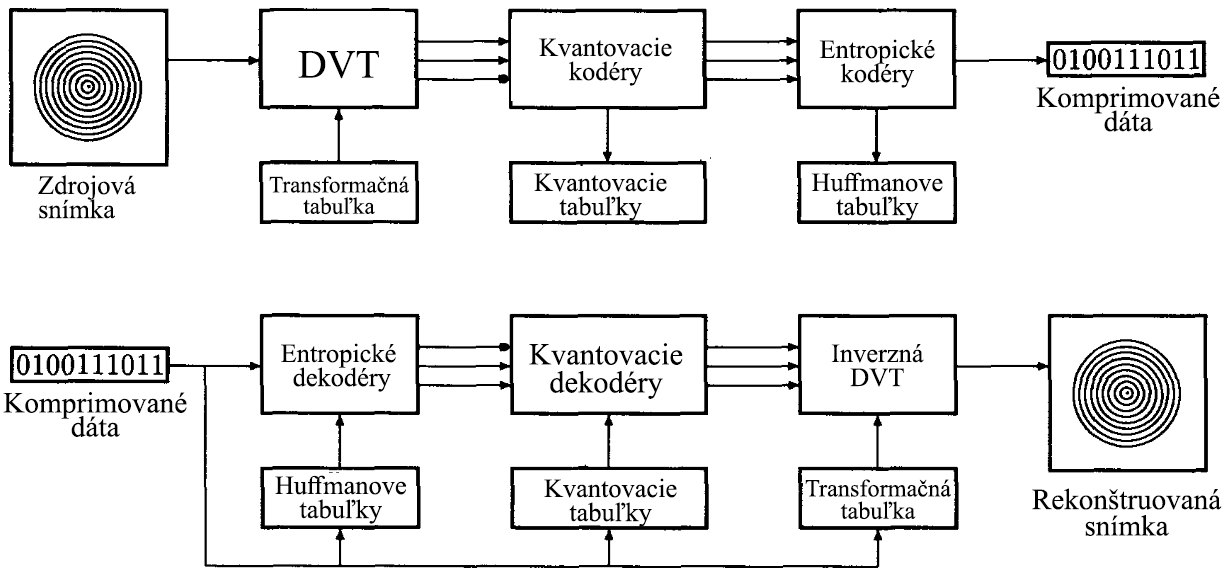
\includegraphics[width=10cm]{obrazky-figures/WSQ_encoder_decoder.png}
    \caption{Diagram WSQ kódera a dekódera \cite{Bradley}}
    \label{obr:WSQ_diagram}
  \end{figure}
  
  \subsection*{Diskrétna vlnková transformácia}
  Prvým krokom v kompresii snímok vo formáte WSQ je diskétna vlnková transfornácia, ktorá prevedie viacúrovňovú dekompozíciu vstupnej snímky na 
  podpásma. Jedna úroveň transformácie je zobrazená na obrázku \ref{obr:DWT_uroven}. Vstupný signál I je rozdelený na podpásma filtrami horného
  a dolného priepustu, pričom prvý pár filtrov spracúva riadky vstupného signálu a zvyšné dva páry filtrov spracúvajú stĺpce vstupného signálu.
  Kombináciou typu filtrov a smeru filtrovania sa získavajú štyri skupiny koeficientov transformácie v rôznych smeroch: 
  \begin{itemize}
    \item \emph{LL} produkuje aproximáciu vstupného signálu
    \item \emph{HL} produkuje detaily vo vertikálnom smere
    \item \emph{LH} produkuje detaily v horizontálnom smere
    \item \emph{HH} produkuje detaily v diagonálnom smere.
  \end{itemize}
  Po každom filtri sa signál podvzorkuje s faktorom 2, čo znamená, že výsledná veľkosť vektoru jednotlivých koeficientov bude štvornásobne menšia
  z dôvodu podvzorkovania ako riadkov, tak stĺpcov vstupného signálu.

  Jednotlivé podpásma je možné naďalej kaskádovať cez takúto transformačnú banku, kým sa nedosiahne požadovaná úroveň rozkladu vstupného signálu.
  Formát WSQ aplikuje viacúrovňovú dekompozíciu podpásem naznačenú na obrázku \ref{obr:WSQ_DWT_dekompozicia}.
  \begin{figure}[]
    \centering
    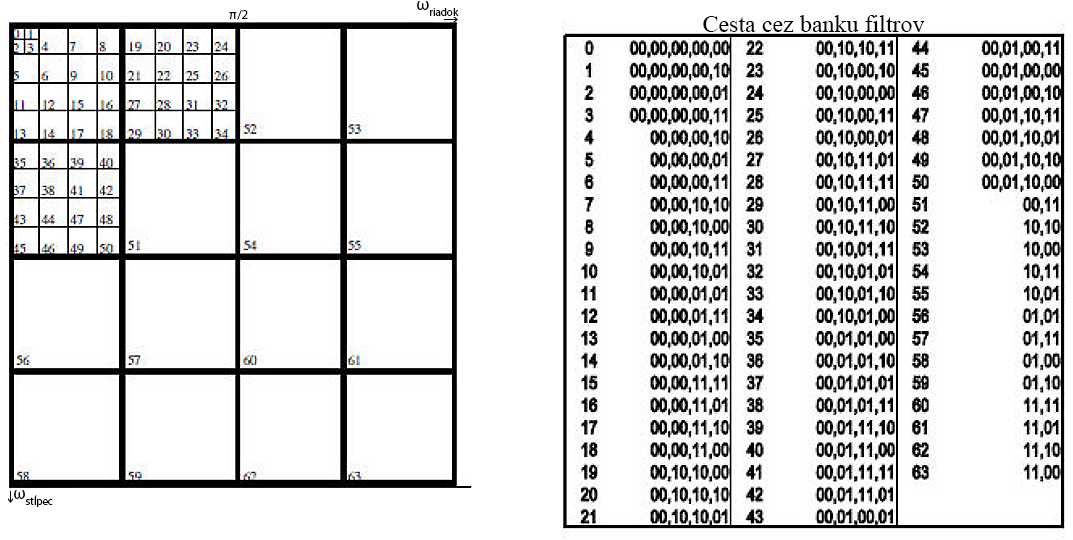
\includegraphics[width=12cm]{obrazky-figures/WSQ_DWT_subband_decomposition.png}
    %//TODO: prekreslit tento obrázok vo vyssej kvalite a podla L/H oznaceni, ktore som vyuzil v tejto sekcii namiesto a_xx ako je vo wsq specifikacii
    \caption{Dekompozícia podpásem vo formáte WSQ.}
    \label{obr:WSQ_DWT_dekompozicia}
  \end{figure}

  \begin{figure}[]
    \centering
    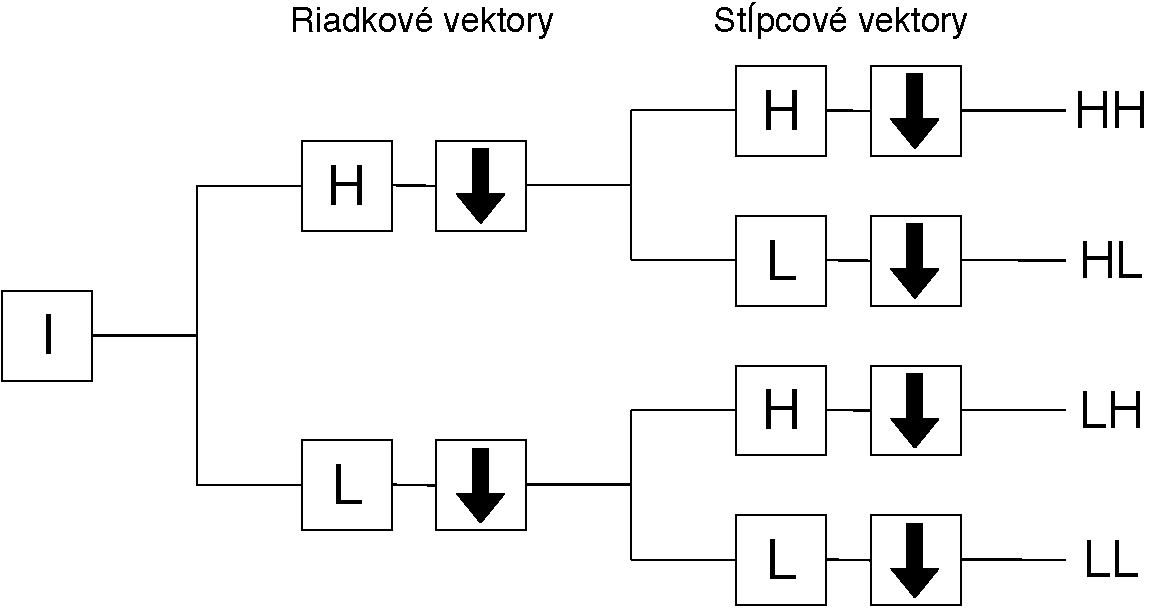
\includegraphics[width=10cm]{obrazky-figures/DWT_level.pdf}
    \caption{Diagram zobrazujúci jednu úroven rozkladu vstupnej snímky do korešpondujúcich podpásem, kde bloky H predstavujú filtre s horným priepustom,
    bloky L filtre s dolným priepustom, bloky so šípkou nadol značia podvzorkovanie a blok I je vstupný signál.}
    \label{obr:DWT_uroven}
  \end{figure}

  \subsection*{Kvantovanie}
  Proces kvantovania je spôsob diskretizácie vstupného signálu. V tomto prípade sa jedná o diskretizáciu koeficientov určených diskrétnou vlnkovou
  transformáciou v predošlom kroku. Jednotlivé koeficienty podpásem získaných transformáciou sú uniformne kvantované v rámci každého podpásma.
  Znamená to, že každé podpásmo môže mať vlastné hodnoty kvantovacieho kroku a šírky kvantovacej \uv{nádoby} (kvantovaného rozsahu). 
  % //TODO: "quantization bin" do slovenciny namiesto "kvantovacia nádoba"...

  Kvantovanie a jeho reverzná operácia pre dekódovanie komprimovaných snímok sú dané vzťahmi \ref{rov:kvantovanie} a \ref{rov:kvantovanie_reverz}:
  \begin{equation}
    p_k(m,n) =
    \begin{cases}
      \lfloor \frac{a_k(m,n) - Z_k / 2 }{Q_k} \rfloor + 1, & a_k(m,n) > Z_k/2 \\
      0, & -Z_k/2 \leq a_k(m,n) \leq Z_k/2 \\
      \lceil \frac{a_k(m,n) + Z_k / 2 }{Q_k} \rceil - 1, & a_k(m,n) < -Z_k/2 \\
    \end{cases}
    \label{rov:kvantovanie}
  \end{equation}
  \begin{equation}
    \hat{a}_k(m,n) = 
    \begin{cases}
      (p_k(m,n) - C)Q_k + Z_k/2, & p_k(m,n) > 0 \\
      0, & p_k(m,n) = 0 \\
      (p_k(m,n) + C)Q_k - Z_k/2, & p_k(m,n) < 0\\
    \end{cases}
    \label{rov:kvantovanie_reverz}
  \end{equation}
  kde subskript $k$ označuje $k$-te podpásmo, $a_k(m,n)$ označuje koeficient v danom podpásme, $Z_k$ je šírkou nulovej kvantovacej nádoby,
  $Q_k$ je šírkou nenulovej kvantovacej nádoby a $C$ je centrom kvantovacích nádob. $C$ je špecifikáciou daný ako $C = 0,44$ pre najnovší enkodér,
  pričom $Z_k$ a $Q_k$ sa získa výpočtom rozptylu jednotlivých podpásem.


  \subsection*{Entropické kódovanie}
  Ako predpoklad kódovania špecifikácia určuje rozdelenie snímky do minimálne troch blokov, kde prvá hranica je medzi podpásmami 18 a 19 a druhá
  hranica medzi podpásmami 51 a 52. Je to z dôvodu zabezpečenia progresívneho prenosu, čo znamená, že po sebe nasledujúce bloky pridávajú detaily
  snímky. Vďaka charakteristike dekompozície pomocou DWT prevedenej v prvom kroku kompresie je možné preniesť najvyššiu úroveň aproximácie a
  orientovaného detailu snímky, z čoho je možné rekonštruovať aproximačnú snímku nižšej úrovne. Rozdelením podpásem do blokov na týchto konkrétnych
  indexoch zabezpečí možnosť graduálnej rekonštrukcie snímky pridávaním detailov nižsej úrovne dekompozície,
  ako je zrejmé zo snímky \ref{obr:WSQ_DWT_dekompozicia}. Rozdelenie do viacerých, než troch blokov je vo WSQ tiež možné.

  Pre bezstratovú kompresiu kvantovaných dát sa používa Huffmanovo kódovanie, ktoré využíva početnosť jednotlivých symbolov v datasete pre 
  generovanie čo najkratších kódových slov pre najpočetnejšie symboly. V prípade WSQ sú symbolmi kvantované koeficienty a nulové reťazce
  rôznych dĺžok. WSQ definuje aj špeciálne symboly pre koeficienty a nulové reťazce, ktoré presahujú rozsah kódovacej tabuľky a tieto sú označované
  riadiacou (escape) sekvenciou.

\chapter{Návrh aplikácie} \label{kap:navrh_appky}
  \section{Požiadavky}
  Medzi základné požiadavky pre zobrazovač a editor snímok odtlačkov prstov patria podpora štandardných formátov využívaných
  pre ukladanie snímok odtlačkov prstov (napr. WSQ, PNG, BMP),
  detekcia singularít, markantov a triedy odtlačku, ukážka filtrov využívaných pri predspracovávaní odtlačkov prstov.

  Vzhľadom na účel aplikácie, a to demonštrácia spracovania odtlačkov prstov, je vhodné ju navrhnúť tak, aby bola prenositeľná a mala prehľadné 
  grafické rozhranie pre jednoduché využitie študentmi a výskumníkmi nezávisle od ich preferovaného systému.

  \section{Architektúra aplikácie}
  Aplikácia je napísaná v jazyku Python 3.5.3 s využitím väzby na Qt toolkit pre programovanie grafických rozhraní pomocou PyQt.
  % //TODO zistit, ci sa pouzije cx_freeze na freeznutie aplikacie do spustitelneho suboru
  

  \section{Grafické rozhranie}
  Grafické rozhranie pozostáva z ovládacieho panelu, pomocou ktorého je možné vykonávať operácie nad snímkami a z ukážky súčasne
  spracovávaného odtlačku prsta. Ukážka reflektuje úkony vykonávané na snímke pomocou ovládacieho panelu.

  Ovládací panel obsahuje výber jednotlivých filtrov, transformácii a iných úkonov. %//TODO: toto dopisat

  \section{Automatická analýza}
  Režim automatickej analýzy sa drží zaužívaných postupov naznačených v kapitole \ref{kap:odtlacok}. Kroky predspracovania zahŕňajú 
  normalizáciu snímky, filtrovanie Gaborovým filtrom, následnú extrakciu orientácií papilárnych línií, binarizáciu a stenčenie línií.
  
  %Predspracovanie snímky sa začne normalizáciou histogramu

  %\begin{figure}[]
  %  \centering
  %  % //TODO: nakreslit flowchart analýzy
  %  
\includegraphics[width=5cm, height=5cm]{obrazky-figures/placeholder.pdf}
  %  \caption{Kroky automatického analyzátora}
  %  \label{obr:analysis_flowchart}
  %\end{figure}
